\cotefile{37}
\scanpage{3}
SGA : Manuscripts à frapper

\diagram{\begingroup\small
\(\begin{array}{llll}
\text{\deleted{SGA 1}} & \text{\deleted{Index notations et terminologique:}} & & \text{\deleted{\uline{10} p}}\\
\text{SGA \unsure{\deleted{2}4|\deleted{4}2}} & \text{\tikz[remember picture,baseline=(sgaiv.base)]\node[inner sep=0pt] (sgaiv) {Exp IV (fin)};} & \text{Verdier} & \text{\uline{\unsure{5|\deleted{3}5}0}}\\
& \text{Exp V} & \text{Verdier} & 80\smash{\raisebox{-1.5em}{\handwritten{\(\left.\rule{0pt}{3.6em}\right\}\)}}}\smash{\raisebox{-3em}{\handwritten{\(\left.\rule{0pt}{6.6em}\right]\)}}}\\
& \text{Exp VI (fin)} & \text{Verdier} & 50\\
& \text{Exp VI B} & \text{S\deleted{q}aint Donat} & \text{\unsure{\deleted{5}1|\deleted{1}5}0}\\
& \text{\shortstack[l]{Tables des matières pour les trois\\ volumes, index}} & & 30\\
& \text{Appendice à \unsure{XVII|\deleted{I}XVII}} & \text{Saint Donat} & 10\\
\text{SGA 5} & \text{Exp IV} & ? & 100\ ?\\
& \text{\tikz[remember picture,baseline=(sgavii.base)]\node[inner sep=0pt] (sgavii) {Exp VII};} & \text{Jouanolou} & \text{\uline{50}}\\
& \text{\tikz[remember picture,baseline=(sgaxi.base)]\node[inner sep=0pt] (sgaxi) {Exp XI};} & \text{Bucur} & \text{\uline{70}}\\
& \text{Exp XII} & \text{Bucur} & 100\smash{\raisebox{-0.65em}{\handwritten{\(\left.\rule{0pt}{2em}\right]\)}}}\\
& \text{Exp XIV} & \text{Grothendieck} & 20\\
& \text{\shortstack[l]{Introduction, table des matières,\\ index}} & & 15\\
\text{\deleted{SGA 6}} & \text{\deleted{Exp XI}} & \text{\deleted{Ferrand}} & \text{\deleted{70 ?}}\\
& \text{\deleted{Table des matières, index}} & & \text{\deleted{10}}\\
\text{SGA 7} & \text{Exp I à \deleted{II}IV} & ? & 120\ ?\\
& \text{Exp \deleted{V}V} & \text{Mme Raynaud} & \text{\tikz[remember picture,baseline=(raynaudcount.base)]\node[inner sep=2pt] (raynaudcount) {30};}\\
& \text{\tikz[remember picture,baseline=(sgarim.base)]\node[inner sep=0pt] (sgarim) {Exp VI};} & \text{Rim} & \text{\tikz[remember picture,baseline=(rimcount.base)]\node[inner sep=2pt] (rimcount) {\uline{70}};}\\
& \text{\shortstack[l]{Introduction, table des matières,\\ index}} & & 15
\end{array}\)
\endgroup}
% Right margin, opposite the cancelled SGA 1 row.
\margin{\handwritten{--- \unsure{tel|Cl} Saarbach}}
% Right margin, opposite the bracket joining SGA 5 Exp XII and Exp XIV.
\margin{\handwritten{--- \uline{écrire Bucur}}}
% Right margin, opposite the framed SGA 7 counts 30 and 70.
\margin{\handwritten{\uline{écr. Deligne}}}
% Pencil strokes are anchored to their source table rows; the counts remain typed.
\handwritten{\figure{\begin{tikzpicture}[remember picture,overlay]
\draw ([xshift=-.8cm,yshift=-.45cm]sgaiv.south west) -- ([yshift=-.08cm]sgaiv.south west) -- ([yshift=-.08cm]sgaiv.south east);
\draw ([xshift=-1.05cm,yshift=-.3cm]sgavii.west) -- (sgavii.west);
\draw ([xshift=-.95cm,yshift=-.4cm]sgaxi.west) -- (sgaxi.west);
\draw ([xshift=-1.4cm,yshift=-.55cm]sgarim.west) -- (sgarim.west);
\draw (raynaudcount.north west) -- (raynaudcount.north east) -- (rimcount.south east) -- (rimcount.south west) -- cycle;
\draw ([xshift=-1pt,yshift=1pt]raynaudcount.north west) -- ([xshift=1pt,yshift=1pt]raynaudcount.north east) -- ([xshift=1pt,yshift=-1pt]rimcount.south east) -- ([xshift=-1pt,yshift=-1pt]rimcount.south west) -- cycle;
\draw ([xshift=-3pt]raynaudcount.south west) -- ([xshift=1pt,yshift=-1pt]raynaudcount.south east);
\end{tikzpicture}}}

NB Les chiffres soulignés correspondent à des exposés dont le manuscrit est disponible dès maintenant; ceux suivis d'un signe ? à ceux dont il n'est pas certain qu'ils seront rédigés. En plus de la frappe d'exposés, tables de matières, index, il y a pour chacun des cinq séminaires envisagés un certain travail de mise\deleted{\unsure{r}} au point (\unsure{correction|corection} de fautes de frappe et autres erreurs, insertion de notes de bas de page etc), représentant un travail variable d'un séminaire à l'autre. Il faudrait sans doute fixer un forfait pour chacun d'eux, pour la rénumération de la sécrétaire, après examen avec elle des corrections à faire ...

Il y a actuellement dans les 250 pages prêtes pour la frappe. J'espère que dans les deux ou trois mois qui v\unsure{\deleted{ei}ie|\deleted{ie}ei}nnent, il y aura aussi les env. \unsure{\deleted{3}2|\deleted{2}3}00 pages qui manquent encore pour SGA 4 (qui sont déjà partiellement rédigés ...), ce qui ferait dans les 450 à 500 pages à frapper pour les cinq à six mois qui viennent. Cependant je ne peux le garantir, cela dépendra de Mr. Verdier, qui est à Brandeis cette année. Je me mets en rapport avec lui ces jours-ci.
% archive sheet number: 2

\scanpage{4}
\begin{flushright}
Massy le 3.11.1970\\
\end{flushright}
Chère Madame Michon,\\

Je m'aperçois que dans les exemplaires SGA d'archives que j'ai emportés de chez vous, il manque les suivants:
\[
\text{SGA 4 XVII}\quad,\quad\text{SGA 4 VI (première partie)}
\]

D'autre part j'ai besoin de ces exemplaires pour faire faire l'édition photooffset en préparation. Pourriez vous me les retrouver ?

Bien cordialement\\
% archive sheet number: 3

\scanpage{5}
\begin{flushright}
Massy le 3.11.1970\\
\end{flushright}
Cher Deligne,\\

Pourrais-tu me dire si tu as terminé de regarder l'exposé de Rim SGA 7 VI, et si oui, me l'envoyer avec tes commentaires (sinon, me dire si tu as l'intention de le regarder et quand) ?

J'ai demandé à Mlle Altazin, qui a tapé ton exposé SGA 4 XVIII, de te l'envoyer avec le manuscrit, pour que tu le corriges. Pourrais-tu me dire si tu l'as reçu et si tu as l'intention de faire les corrections ? Quand elles seront faites, ou si tu ne veux pas les faire, envoyes moi le texte au net stp.

As-tu eu des nouvelles de Ferrand pour SGA 6 XI ?

Bien cordialement\\
% archive sheet number: 4

\scanpage{7}
\mspage{(ix)}
de ces questions que j'avais fait ailleurs. Ainsi, je me suis trouvé travailler pendant trois ans dans une institution alors qu'elle participait à mon insu à un mode de financement que je considère comme profondément immoral et extrêmement dangereux. Etant à présent seul à avoir cette opinion parmi mes collègues à l'IHES, ce qui a condamné à l'échec mes efforts pour obtenir la suppression des subventions militaires du budget de l'IHES, j'ai pris la décision qui s'imposait et quitte l'IHES le 30 Septembre prochain, et suspends également toute collaboration scientifique avec cette Institution, aussi longtemps qu'elle continuera à accepter de telles subventions. Monsieur L. Motchane, directeur de l'IHES, s'est déclaré d'accord pour qu'à partir du 1\textsuperscript{er} Octobre 1970, l'IHES ne diffuse plus les textes mathématiques dont je suis auteur, ou faisant partie du Séminaire de Géométrie Algébrique du Bois Marie. Comme il a été dit plus haut, la diffusion de ce Séminaire va être assurée par la maison Julius Springer, dans la série des Lecture Notes. Je suis heureux de remercier ici la maison Springer et Monsieur K. Peters pour l'aide efficace et courtoise qu'ils m'ont apportée pour rendre possible cette publication, en se chargeant en particulier de la frappe pour la photooffset des nouveaux exposés rajoutés aux anciens séminaires, et des exposés manquants des séminaires incomplets.

\begin{flushright}
Massy, Août 1970\\
\end{flushright}
% archive sheet number: 6

\scanpage{9}
\begin{flushright}
\handwritten{16 Juillet .}\\
\end{flushright}
Cher Grothendieck,\\

Voici la nouvelle rédaction de \handwritten{4}.\handwritten{10}.\handwritten{6}.

En relisant le n\textsuperscript{o} \handwritten{9} de S.G.A \handwritten{4} IV j'ai trouvé les broutilles suivantes :

p. \handwritten{149} l. \handwritten{16} lire \(E'\handwritten{\vee} E'' = E\)

p. \handwritten{158} l. \handwritten{5} lire \(s\varepsilon\operatorname{Hom}(e_E,G)\)

p. \handwritten{158} compléter le diagramme \handwritten{9}.\handwritten{3}.\handwritten{6}.\handwritten{2}

p. \handwritten{159} l. \handwritten{15} lire ``le foncteur \(\handwritten{\sigma}\) composé de

Dans les n\textsuperscript{o} \handwritten{10} et suivant j'ai trouvé

p. \handwritten{2} l. -\handwritten{7} lire ``doù l'assertion ''

p. \handwritten{14} l. \handwritten{5} lire \(\handwritten{\mathscr{H}}\mathrm{om}_A\)

p.\handwritten{14} l. \handwritten{17} itou .

% Left margin: the two sloping underlined words stand to the left of the vertical paragraph mark.
\reversemarginpar
\margin{\handwritten{\figure{
\begin{tikzpicture}[x=.85cm,y=.85cm]
\node[rotate=36,anchor=base west,inner sep=0pt] at (.15,.82) {\uline{demander}};
\node[rotate=36,anchor=base west,inner sep=0pt] at (.35,.35) {\uline{Messing}};
\draw (2.26,.35) -- (2.26,1.62);
\end{tikzpicture}}}}
\normalmarginpar
Enfin , désagréable surprise , je me suis aperçu qu'il manquait le n\unsure{\deleted{?}\handwritten{\textsuperscript{o}}|\handwritten{\textsuperscript{o}}} \handwritten{14} dans les notes que tu m'as envoyés (Modules sur un topos défini par recollement ). Je me souviens avoir rédigé ce numéro et je pense bien te l'avoir donné . En tout cas je ne l'ai pas dans mes papiers . J'espère que ce numéro ne s'est pas perdu .

\begin{flushright}
Bien à toi\\
\handwritten{J. \unsure{L|V}}\\
\end{flushright}
% archive sheet number: 8

\scanpage{10}
\uline{Exercice} \handwritten{4}.\handwritten{10}.\handwritten{6} . Soient \(S\) un \(\underline{U}\)-site dont la topologie est moins fine que la canonique , \(\underline{\deleted{\unsure{S}}\handwritten{M}}\) une partie de \(\mathrm{Fl}(S)\) possédant les propriétés suivantes :

 a) Les morphismes de \(\underline{M}\) sont quarrables (I \handwritten{10}.\handwritten{3}) et \(\underline{\unsure{\deleted{S}M|\deleted{M}S}}\) est stable par changement de base.

% The overtyping-order doubt marked in a) also applies to the repeated form in b).
 b) \(\underline{\deleted{S}M}\) contient les flèches identiques et est stable par composition .

 c) Une flèche \(u:X\to Y\) telle qu'il existe une famille couvrante \(Y_i\to Y\) , avec les \(X\times_Y Y_i\to Y_i\) dans \(\underline{M}\) , est elle-même dans \(\underline{M}\) .

 d) Pour tout objet \(X\) , toute famille couvrante de \(X\) est raffinée par une famille couvrante \((f_i:X_i\to X)\) où les \(f_i\) sont dans \(\underline{M}\).

Pour tout objet \(X\) , \deleted{considérons le site}\inserted{notons} \(S(X)\) (``petit site de \(X\)'')%
% Matching handwritten looped insertion signs: attachment in the text and words in the left margin.
\handwritten{
\begin{tikzpicture}[x=1pt,y=1pt,baseline=-1pt]
\draw[line width=.55pt,line cap=round] (0,0) .. controls (1.7,4.8) and (4.2,8.8) .. (5.5,11.3);
\draw[line width=.55pt,line cap=round] (5.5,11.3) .. controls (3.6,10.7) and (3.9,14.2) .. (5.7,14.4) .. controls (8.6,14.4) and (8.6,11.2) .. (5.5,11.3);
\end{tikzpicture}}%
\reversemarginpar
\margin{\handwritten{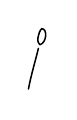
\begin{tikzpicture}[x=1pt,y=1pt,baseline=-2pt]
\draw[line width=.55pt,line cap=round] (0,-1) .. controls (1,4.3) and (2.5,9.1) .. (3.6,13.7);
\draw[line width=.55pt,line cap=round] (4.1,15) .. controls (2.8,15.8) and (3.5,19.6) .. (4.8,20.8) .. controls (7,20.9) and (6.6,15.6) .. (4.1,15);
\end{tikzpicture}}\inserted{le site}}
\normalmarginpar
\deleted{dont la catégorie sous-jacente est}\inserted{constitué par} la sous-catégorie pleine de \(S/X\) formée des objets dont le morphisme structural est dans \(\underline{M}\) , munie de la topologie induite par celle de \(S\) (III \handwritten{3}.\handwritten{1}).

1) Montrer que les familles couvrantes \((f_i:X_i\to X)_{i\varepsilon I}\) où les \(f_i\) sont dans \(\underline{M}\) forment une prétopologie sur \(S\) (II \handwritten{1}.\handwritten{3}) qui engendre la topologie de \(S\) .

2) Pour toute flèche \(u:X\to Y\) de \(S\) , montrer que le foncteur changement de base par \(u\) est un foncteur continu (III \handwritten{1}.\handwritten{1}) de \(S(Y)\) dans \(S(X)\) . \unsure{\(\mathbb{O}\)|\deleted{o}O|\deleted{O}o}n notera
\[
S(u)^{\handwritten{*}}:S(Y)^{\handwritten{\sim}}\to S(X)^{\handwritten{\sim}}
\]
le foncteur correspondant entre les catégorie\handwritten{s} de faisceaux (III \handwritten{1}.\handwritten{2},iv)).

3) Définir une équivalence entre le topos \(S^{\handwritten{\sim}}\) et la catégorie des systèmes
\[
(F_X)\ (X\varepsilon\operatorname{ob}S)\quad,\quad(\handwritten{\varphi_u})\ (u\varepsilon\mathrm{Fl}\ S)
\]
formés d'objets \(F_X\varepsilon\operatorname{ob}S(X)^{\handwritten{\sim}}\) , et pour toute flèche \(u:X\to Y\) dans \(S\) , d'un morphisme \(\handwritten{\varphi}_u:S(u)^{\handwritten{*}}(F_Y)\to F_X\) , ces systèmes
% archive sheet number: 9

\scanpage{11}
étant soumis à une condition de transitivité pour un composé \(v_{\unsure{\circ|o}}u\) de flèches de \(S\) , et à la condition que \(u\varepsilon\underline{M}\) implique que \(\handwritten{\varphi}_u\) soit un isomorphisme .

\handwritten{3}) Définir des foncteurs ``restrictions '' et `` prolongement ''
\[
\operatorname{Res}_X:(S_{\handwritten{/}X})^{\handwritten{\sim}}\to S(X)^{\handwritten{\vee}}\ ,\quad
\operatorname{Prol}_X:S(X)^{\handwritten{\sim}}\to(S_{\handwritten{/}X})^{\handwritten{\sim}}\ ;
\]
montrer que \(\operatorname{Res}_X\) commute aux limites inductives et aux limites projectives et que \(\operatorname{Prol}_X\) est \uline{pleinement fidèle} , son image essentielle étant formée des faisceaux \(F\) tels que \(\handwritten{\varphi}_u\) soit un isomorp\unsure{\deleted{g}h|\deleted{h}g}isme pour toute flèche \(u\) de \deleted{du} \(S_{\handwritten{/}X}\) .

\handwritten{4}) Définir un isomorphisme d'adjonction faisant de \(\operatorname{Res}_X\) l'adjoint à droite de \(\operatorname{Prol}_X\) . En conclure qu'il existe un morphisme de topos
\[
f:S(X)^{\handwritten{\sim}}\to(S_{\handwritten{/}X})^{\handwritten{\sim}}
\]
tel que \(f^{\handwritten{*}}=\operatorname{Res}_X\) et que le foncteur \(f^{\handwritten{*}}\) admet un adjoint à gauche \(f_!=\operatorname{Prol}_X\) . Montrer que \(\operatorname{Prol}_X\) transforme les faisceaux abéliens en faisceaux abéliens . Montrer que \(f:S(X)^{\handwritten{\sim}}\handwritten{\longrightarrow}(S_{\handwritten{/}X})^{\handwritten{\sim}}\) est un \uline{plongement} de topos (\handwritten{9}.\handwritten{1}.\handwritten{1}) et que par suite ``le petit topos '' \(\handwritten{S(X)^{\sim}}\) est \deleted{un sous-topos (\unsure{9.1}} équivalent à un sous-topos du ``gros topos '' \((S_{\handwritten{/}X})^{\handwritten{\sim}}=S^{\handwritten{\sim}}_{\handwritten{/}X}\) .

\handwritten{5}) Soit \(F\) un faisceau abélien flasque de \(S^{\handwritten{\sim}}_{\handwritten{/}X}\) (V \handwritten{4}) . M\textsuperscript{O}ntrer que \(\operatorname{Res}_X F\) est \(S(X)\)-acyclique\handwritten{
\begin{tikzpicture}[x=1cm,y=1cm,baseline=0pt]
\draw[line width=.5pt] (0,-.18) -- (.13,.42);
\draw[line width=.5pt] (.13,.42) .. controls (.09,.47) and (.14,.53) .. (.17,.49) .. controls (.20,.45) and (.16,.40) .. (.13,.42);
\end{tikzpicture}}%
% The cross-reference and its matching looped mark stand in the LEFT margin.
\reversemarginpar\margin{\handwritten{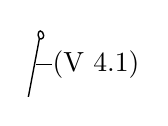
\begin{tikzpicture}[x=1cm,y=1cm,baseline=(ref.base)]
\draw[line width=.5pt] (0,-.22) -- (.14,.52);
\draw[line width=.5pt] (.14,.52) .. controls (.10,.58) and (.14,.65) .. (.18,.60) .. controls (.22,.54) and (.17,.50) .. (.14,.52);
\draw[line width=.4pt] (.10,.19) -- (.30,.19);
\node[anchor=west,inner sep=0pt] (ref) at (.30,.19) {\inserted{(V 4.1)}};
\end{tikzpicture}}}\normalmarginpar . En déduire que pour tout faisceau abélien \(F\) de \(S^{\handwritten{\sim}}_{\handwritten{/}X}\) et tout entier \(q\) , le groupe \(H^q(X,F)\) (cohomologie calculée dans \(S^{\handwritten{\sim}}_{\handwritten{/}X}\) ) est canoniquement isomorphe au groupe \(H^q(X,\operatorname{Res}_X F)\) (cohomologie calculée dans \(S(X)^{\handwritten{\sim}}\) ) .

\handwritten{6}) Déduire de 5) que pour tout faisceau abélien \(G\) \deleted{sur} de \(S(X)^{\handwritten{\sim}}\) et tout entier \(q\) le groupe \(H^q(X,G)\) \deleted{(resp.} (cohomologie calculée dans \(S(X)^{\handwritten{\sim}}\) ) est canoniquement isomorphe aux groupes \(H^q(X,f_{\handwritten{*}}G)\) et \(H^q(X,\operatorname{Prol}_X G)\) (cohomologie calculée dans \(S^{\handwritten{\sim}}_{\handwritten{/}X}\) ) .
% archive sheet number: 10

\scanpage{12}
\uline{Exercice} \handwritten{4}.\handwritten{10}.\handwritten{7} . On reprend les hypothèses et les notations de l'exercice \handwritten{4}.\handwritten{10}.\handwritten{6} . On suppose de plus que \(\underline{M}\) possède la propriété suivante :

(Et) Pour tout couple de flèches composables \(u\) et \(v\) de \(\mathrm{Fl}\ S\) , les \deleted{ces} propriétés \(u_{\unsure{\circ|o}}v\varepsilon\underset{\handwritten{\deleted{\unsure{m|M}}}}{\underline{M}}\) et \(u\varepsilon\underline{M}\) impliquent \(v\handwritten{\varepsilon}\underline{M}\) .

1) Montrer que pour toute flèche \(u:X\to Y\) , le foncteur de changement de base par \(u\) est un morphisme \deleted{du topos} \(S(u)\) du site \(S(X)\) dans le site \(S(Y)\) . En d'autres termes , montrer que \(S(u)^{\handwritten{*}}:S(Y)\to S(X)\) est exact à gauche .

2) Montrer que \(\operatorname{Prol}_X:S(X)^{\handwritten{\vee}}\to(S_{\handwritten{/}X})^{\handwritten{\sim}}\) est exact à gauche . En déduire qu'il existe un morphisme de topos
\[
g:S^{\handwritten{\sim}}_{\underset{\handwritten{\deleted{\unsure{u|m}}}}{\handwritten{/}}X}\to S(X)^{\handwritten{\sim}}
\]
tel que \(g^{\handwritten{*}}=\operatorname{Prol}_X\) et \(g_{\handwritten{*}}=\operatorname{Res}_X\) . Montrer que \(g\) est une rétraction du plongement \(f\) i.e qu'on a \(g_{\circ}f\handwritten{\simeq}\operatorname{id}_{S(X)}\) et qu'on a un morphisme ``d'adjonction'' (entre morphismes de topos ) \(\operatorname{id}_{S^{\handwritten{\sim}}_{\handwritten{/}X}}\handwritten{\longrightarrow} f\circ g\) .

\handwritten{3}) Montrer que les conclusion de \handwritten{1}) et \handwritten{2}) ne sont plus valables lorsqu'on ne fait pas l'hypothèse (Et) . (\unsure{\deleted{p}P|\deleted{P}p}rendre pour \(S\) la catégorie des schémas \unsure{\deleted{,}m|\deleted{m},}unie de la topologie f.p.p.f. (fidèlement plate et de présentation finie \handwritten{[} S.G.A. \handwritten{3} IV \handwritten{]} ) et pour \(\underline{M}\) les morphismes \deleted{fidèlement} plats et de p\unsure{\deleted{é}r|\deleted{r}é}ésentation finie ).

\handwritten{4}) Acheter une médaille en chocolat pour les rédacteurs .
% archive sheet number: 11

\scanpage{13}
\begin{flushright}
Massy le 23.6.1971\\
\end{flushright}
\unsure{Cher} Verdier,\\

Merci pour ta lettre du 23 Mai. C'est dommage que \illegible{1} \unsure{ne} m'aies pas \unsure{ènvoyé|ênvoyé} ce malheureux exer 4.10.6, cela a\unsure{u|n|r}\illegible{1} \unsure{permis} d'envoyer enfin à l'imprimeur \unsure{\deleted{c}l|\deleted{e}l|\deleted{l}c|\deleted{l}e|d}e fascicule 1 de \unsure{SGA} 4. La personne qui a frappé le texte termine mainte\illegible{1} \unsure{e}ll\unsure{\deleted{l}e|\deleted{e}l}\deleted{\illegible{1}} partira en vacances et Springer rend la machine \unsure{qu'elle} avait en location, faute d'autres manuscrits. \unsure{Cela} remet donc la publication même de ce \unsure{fascimle|fascicule} sine \unsure{d|l}ie.

Bien cordialement\\
% archive sheet number: 12

\scanpage{15}
\begin{flushright}
Massy le 18.5.1971\\
\end{flushright}
Cher Verdier,\\

Je ne trouve pas une minute pour m'occuper de la réédition de SGA 4. Saavedra m'a un peu aidé, \unsure{pour} faire un index pour le Chap IV , par.9 à 13. Mais on est bloqué faute d'avoir les deux appendices de Deligne (assez, de points, image inverse d'un plat), qu'il faudrait donner à la frappe. Les\deleted{\unsure{r}}as-tu, et si oui, peux-tu les envoyer pourlla frappe ? D'autre part, peux-tu envoyer une version corrigée de l'exercice 4.10.6 (médaille chocolat), j'ai \unsure{entièrement} oublié ce qui était canulé. C'est un exercice qui sert tout le temps (!), i\unsure{\deleted{o}l|\deleted{l}o} ne devrait donc pas être question de le vider. Il doit y avoir quelque chose de vrai à mettre à la place du faux ...

Si tu en as marre de t'occuper de la mise au point ``définitive'' de SGA 4, je ne pourrais t\unsure{\deleted{e}'|\deleted{'}e}en blâmer. Je voudrais alors des instructions sur ce qu'il faut faire - je suis disposé à le laisser incomplet et dégueulasse, plûtôt que d'avoir à \deleted{une} y consacrer un jour ou deux aux dépens du boulot survie, infiniment plus important. Pourrais-tu demander à Artin ce qu'il faut faire avec les exposés après VI - j'ai des tas de notes d'errata, footnotes améliorations diverses - d'en faire des instructions compréhensibles pour une dactylo demanderait des jours de travail. Veut-il que je lui envoie mon paquet de notes ?
% archive sheet number: 14

\scanpage{16}
\begin{flushright}
Massy le 3.11.1970\\
\end{flushright}
Cher Verdier,\\

Ne m'étant guère occupé de Math depuis trois mois, je suis un peu perdu pour SGA 4. Si je me rappelle bien, tu as rédigé ou es en train de rédiger les parties suivantes, qui sont exactement ce qui manque pour que SGA 4 soit complet:
\diagram{\(\begin{array}{ll}
\text{\deleted{IV,}} & \text{\deleted{par.9 et suivants}}\\
\text{V} & \\
\text{VI} & \text{par.5 et suivants}
\end{array}\)}

Si je me rappelle bien, \unsure{\deleted{IV}VI|\deleted{VI}IV} était en fait terminé d'être rédigé, \unsure{\(\mathbb{il}\)|il} fallait seulement y apporter quelques modifications dont on avait discuté avant ton départ. De plus, je pense que tu as avec toi l'exposé
\[
\text{VI B}
\]
de Saint Donat, et je t'envoie également l'Appendice à XVII du même, dont j'avais apparemment lu les premières pages. P\(\mathbb{o}\)urrais tu me le renvoyer (ou le renvoyer à St Donat) avec tes annotations et commentaires ?

Tu dois avoir un\deleted{e} exemplaire du tirage de XVII; le XVIII n'a pas été tapé sur \unsure{\(\mathbb{S}\)|\deleted{s}S|\deleted{S}s}tencils, mais directement sur papier pour offset; \unsure{\deleted{il}la|\deleted{la}il} frappe est terminée, et Deligne est censé la corriger.

Ecris-moi stp où tu en es avec ta part de rédaction, et avec la lecture de VI B . \deleted{S\unsure{\^{r}|\^{t}|î}inger} Pour des raisons techniques, ce serait bien agréable si les textes V,VI,\(\mathrm{VI}_{\mathrm{B}}\) pouvaient être disponibles dans les deux, trois mois qui viennent. Dis-moi en tous cas si tu as l'intention de terminer, et si oui, quand tu penses avoir terminé.

Bien cordialement\\
% archive sheet number: 15

\scanpage{18}
\begin{flushright}\handwritten{\unsure{1.9.3|1.93|1.9.5}, \unsure{1.27|1.23}, 2.9 à reporter au \unsure{n\textsuperscript{o} 3}\unsure{?}\\3.1}\end{flushright}

\(\mathbb{S}\)GA 4 VI

\uline{Sommaire}
\margin{\handwritten{\uline{\unsure{pp|pv|pr}}}}

1. Conditions de finitude pour les objets et flêches d'un topos.\margin{\handwritten{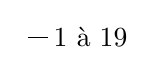
\begin{tikzpicture}[baseline=0,x=.45cm,y=.45cm]\draw (-.7,.12)--(-.15,.12);\node[anchor=west,inner sep=0pt] at (0,.12) {1 à 19};\end{tikzpicture}}}

2. Conditions de finitude pour un topos.\margin{\handwritten{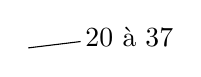
\begin{tikzpicture}[baseline=0,x=.45cm,y=.45cm]\draw (-1.6,-.18)--(-.12,0);\node[anchor=west,inner sep=0pt] at (0,.12) {20 à 37};\end{tikzpicture}}}

3. Conditions de finitude pour un morphisme de topos. \deleted{\handwritten{Cas des \unsure{topos} \unsure{inductifs|induits}}}\margin{\handwritten{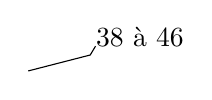
\begin{tikzpicture}[baseline=0,x=.45cm,y=.45cm]\draw (-1.9,-.5)--(-.15,-.05)--(0,.2);\node[anchor=west,inner sep=0pt] at (0,.45) {38 à 46};\end{tikzpicture}}}

\deleted{4. Constructibilité.}\inserted{\handwritten{4. Conditions de finitude pour un topos \inserted{obtenu par} recollement.}}\margin{\handwritten{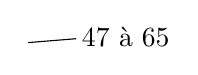
\begin{tikzpicture}[baseline=0,x=.45cm,y=.45cm]\draw (-1.5,-.03)--(-.15,.08);\node[anchor=west,inner sep=0pt] at (0,.12) {47 à 65};\end{tikzpicture}}}
% The pencil divider is immediately beneath the original and replacement item 4.
\noindent
\begin{tikzpicture}[x=\linewidth,y=.4cm]\draw (-.07,0)..controls (.2,-.08) and (.7,.08)..(.96,-.04);\end{tikzpicture}
% The relocation curve remains in the LEFT margin, with its question mark;
% its lower end is beside the circled replacement 5 and its arrowhead points
% to the divider after item 4. The drawing preserves the source's relative geometry.
\reversemarginpar
\margin{\handwritten{\begin{tikzpicture}[x=.55cm,y=.55cm]
\draw[->] (2,-6.5)..controls (-1,-4.6) and (-1,-3.2)..(2,0);
\node at (.05,-1.8) {?};
\end{tikzpicture}}}
\normalmarginpar

\deleted{5}\handwritten{6}. Catégories fibrées et $\underset{\handwritten{\longrightarrow}}{\mathrm{Lim}}$ (rappels).

\deleted{6}\handwritten{7}. Sites et topos fibrés.

\reversemarginpar
\margin{\handwritten{
\begin{tikzpicture}[x=.45cm,y=.45cm]
\draw (1,0)..controls (1,-.8) and (1,-1.0)..(.62,-1.03)
 ..controls (1.2,-1.25) and (.9,-2.1)..(1.16,-2.32);
\end{tikzpicture}}}
\normalmarginpar
\deleted{7}\handwritten{8}. Limites projectives de topos.

\deleted{8}\handwritten{\unsure{8|9}}. Cas des limites projectives filtrantes de topos cohérents par morphismes de transition cohérents: théorèmes de passage à la limite pour la cohomologie.

\noindent\begin{tikzpicture}[baseline=(n.base)]\node[draw,ellipse,inner sep=3pt] (n) {\deleted{9}\handwritten{5}.};\end{tikzpicture} Cohomologie d'une limite inductive de fais\unsure{\deleted{x}c|\deleted{c}x}eaux sur un topos cohérent
% The right edge cuts immediately after the t of cohérent; no full stop is visible.

\reversemarginpar
\margin{\handwritten{\begin{tikzpicture}[x=.25cm,y=.25cm]\draw[line width=2pt] (0,0)--(.04,-.55);\end{tikzpicture}}}
\normalmarginpar
\handwritten{10. Appendice (par P. Deligne). \deleted{Existence de point\unsure{s}} \unsure{\deleted{d'}Un|\deleted{d'Un}} topos cohérent \unsure{a} \inserted{suffisamment de points}\unsure{.}}

\deleted{NB \(\mathbb{B}\)ien sûr \deleted{\unsure{9|8}}\handwritten{8} serait interchangeable avec le bloc \deleted{5}\handwritten{4} à \deleted{8}\handwritten{9}. Mais il me semble plus naturel de mettre dans deux numéros consécuti\unsure{\deleted{s}f|\deleted{f}s}s les deux facettes d\unsure{\deleted{y}u|\deleted{g}u|\deleted{u}y|\deleted{u}g} \unsure{\deleted{b}p|\deleted{p}b|\deleted{l}p|\deleted{p}l}assage à la limite en cohomologie. Bien sû\unsure{\deleted{t}r|\deleted{r}t}, le numéro \deleted{\unsure{9}}\handwritten{8} sera réduit à une ou deux pages, le sorite des conditions de finitude étant déjà fait.}

\deleted{Le n\textsuperscript{\uline{o}} 4 contiendra le sorite des groupes constructibles (au sens groupes finis ou non), des faisceaux de torsion, des notions de constructibilité pour les Modules et complexes de Modules, - y compris les faits spéciaux dans le cas localement noethérien. Je pense que je le rédigerai mais ne le garantis pas. On peut \deleted{à la rigue} laisser t\deleted{\unsure{l|i}}\handwritten{o}mber le n\textsuperscript{\uline{o}}4, ce sera alors moins beau bien sûr ...:}

\deleted{La rédaction qui suit des n\textsuperscript{\uline{o}}s 1 à 3 est ào\unsure{\deleted{p}m|\deleted{m}p}plète, à cela près que je compte y ajouter encore quelques exemples (en particulier un topos localement algébrique non algébrique\inserted{\handwritten{)}}\unsure{,|.} \deleted{un morphisme non cohérent de topos cohérents).}}
\reversemarginpar
\margin{\handwritten{
\begin{tikzpicture}[x=.3cm,y=.3cm]\draw (0,0)--(.35,-2.3);\draw (.15,0)--(.5,-2.3);\end{tikzpicture}}}
\normalmarginpar
\unsure{\inserted{\handwritten{et un topos ayant une famille génératrice formée d'objet\unsure{s} cohérents, qui n'est pas localement algébrique}}}
% The outer unsure on the bottom insertion records live/cancelled-state uncertainty.
% archive sheet number: 17

\scanpage{23}
\reversemarginpar
\margin{\handwritten{SGA 4 $\overline{\text{\uline{VI}}}$ 2}}
\normalmarginpar

\uline{Exercice} \handwritten{2}. . Soi\inserted{en}t $C$ une \deleted{\unsure{\uline{U}-|\uline{U}}}\inserted{petite} catégorie\handwritten{,}\inserted{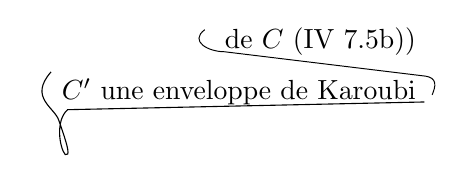
\begin{tikzpicture}[baseline=(kar.base),x=1cm,y=1cm]
\node[inner sep=0pt,anchor=base west] (kar) at (0,0) {$C'$ une enveloppe de Karoubi};
\node[inner sep=0pt,anchor=base east] (ref) at ([yshift=.55cm]kar.east) {\inserted{de $C$ (IV 7.5\handwritten{b))}}};
\draw[line width=.4pt] (-.13,.35) .. controls (-.42,.02) and (-.08,-.10) .. (-.03,-.27)
 .. controls (.10,-.64) and (.11,-.72) .. (.05,-.70)
 .. controls (-.02,-.62) and (-.08,-.27) .. (.08,-.13)
 -- ([xshift=.10cm,yshift=-.13cm]kar.east);
\draw[line width=.35pt] ([xshift=-.25cm,yshift=.15cm]ref.west)
 .. controls ([xshift=-.45cm]ref.west) and ([xshift=-.20cm,yshift=-.13cm]ref.west)
 .. ([yshift=-.13cm]ref.west)
 -- ([xshift=.10cm,yshift=.20cm]kar.east)
 .. controls ([xshift=.28cm,yshift=.18cm]kar.east) and ([xshift=.24cm,yshift=.06cm]kar.east)
 .. ([xshift=.20cm,yshift=-.04cm]kar.east);
\end{tikzpicture}} Montrer que les conditions suivantes sont équivalentes:

(i) La catégorie $\mathrm{Ind}(C)$ (I 8.2) est un \uline{$U$}-topos.

( bis) Le foncteur canonique $\mathrm{Ind}(C)\handwritten{\longrightarrow}\overset{\handwritten{\scriptscriptstyle\wedge}}{C}$ admet un adjoint à droite qui \deleted{commute aux} e\unsure{\deleted{n}s|\deleted{s}n}t ex\(\mathbb{a}\)ct à gauche.

(i ter) Il existe une topologie sur $C$ pour laquelle les faisceaux soient les préfaisceaux ind-représentables.

\figure{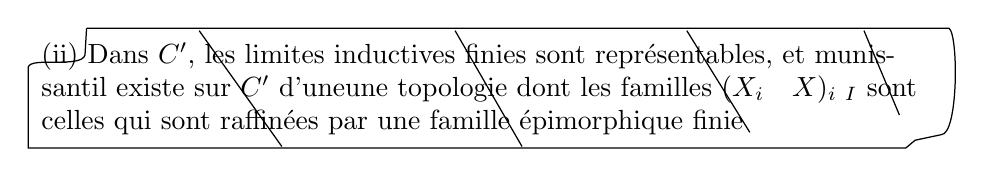
\begin{tikzpicture}
\node[inner sep=4pt,anchor=north west,text width=.94\linewidth] (oldii) at (0,0)
{\deleted{(ii) Dans $C'$, les limites inductives finies sont représentables, \deleted{et munissant}\inserted{il existe sur} $C'$ \deleted{\unsure{d'une}}\inserted{une} topologie dont les familles $(X_i\quad X)_{i\ I}$ sont celles qui sont raffinées par une famille épimorphique finie}};
\draw[line width=.45pt] ([xshift=.72cm,yshift=.03cm]oldii.north west)
 -- ([xshift=-.02cm,yshift=.03cm]oldii.north east)
 .. controls ([xshift=.10cm,yshift=-.05cm]oldii.north east)
 and ([xshift=.10cm,yshift=.15cm]oldii.south east)
 .. ([xshift=-.12cm,yshift=.15cm]oldii.south east)
 -- ([xshift=-.45cm,yshift=.08cm]oldii.south east)
 -- ([xshift=-.57cm,yshift=-.02cm]oldii.south east)
 -- ([xshift=-.02cm,yshift=-.02cm]oldii.south west)
 -- ([xshift=-.02cm,yshift=-.46cm]oldii.north west)
 .. controls ([xshift=.02cm,yshift=-.33cm]oldii.north west)
 and ([xshift=.65cm,yshift=-.48cm]oldii.north west)
 .. ([xshift=.70cm,yshift=-.31cm]oldii.north west)
 -- ([xshift=.72cm,yshift=.03cm]oldii.north west);
\draw[line width=.45pt] ([xshift=2.15cm]oldii.north west)--([xshift=3.20cm]oldii.south west);
\draw[line width=.45pt] ([xshift=5.40cm]oldii.north west)--([xshift=6.25cm]oldii.south west);
\draw[line width=.45pt] ([xshift=-3.35cm]oldii.north east)--([xshift=-2.55cm,yshift=.18cm]oldii.south east);
\draw[line width=.45pt] ([xshift=-1.10cm]oldii.north east)--([xshift=-.65cm,yshift=.40cm]oldii.south east);
\end{tikzpicture}}

(ii) \deleted{Dans $C'$} I\begin{tikzpicture}[baseline=(ell.base),x=1em,y=1ex]
\node[inner sep=0pt,anchor=base] (ell) at (0,0) {l};
\draw[line width=.45pt] (-.19,2.05)--(.19,2.05)--(.19,2.35);
\draw[line width=.45pt] (-.19,-.40)--(.02,-.40)--(.02,-.72);
\end{tikzpicture} existe une topologie sur $C'$ dont les familles couv\unsure{\deleted{a}r|\deleted{r}a}a\unsure{\deleted{t}n|\deleted{n}t}tes sont celles qui so\unsure{\deleted{j}n|\deleted{n}j}t raffinées par une famille épimorphique (ou encore, épimorphique effective universelle ..) \uline{finie}, dans $C'$ les limites \deleted{projectives}\inserted{inductives} finies sont représentables, et le foncteur canonique $C\handwritten{\longrightarrow}\overset{\handwritten{\scriptscriptstyle\sim}}{C}$ \deleted{est} y commute.

(iii) (Si dans $C$ les limites projectives finies sont représentab\deleted{\unsure{l|e}}les,\deleted{\unsure{â|à}} de sorte qu'on peut prendre $C'=C$.) Dans $C$ les limites inductives finies sont représentables, et $C$ satisfait la condition ST) de
\reversemarginpar\margin{\handwritten{$\times$}}\normalmarginpar
I 8.8 f).

(iv) Il existe un topos $E$ engendré par sa sous-catégorie pleine
\reversemarginpar\margin{\handwritten{$\times$}}\normalmarginpar
$E_{\mathrm{PF}}$ (\quad\quad), et une équivalence de catégories $C'\handwritten{\approxeq}E_{\mathrm{PF}}$.

De plus, \deleted{la topologie} si ces conditions sont satisfaites, la topologie postulée dans (i ter) est nécessairement celle décrite dans (ii), et le topos $E$ postulé dans (iv) est nécessairement équivalent à $\mathrm{Ind}(C)$. Ce topos est donc parfait si et seulement si \inserted{dans} $C'$ \deleted{est} les limites projectives finies sont r\unsure{\deleted{r}e|\deleted{e}r}présentables.
% archive sheet number: 22

\scanpage{24}
% letterhead
\noindent\begin{minipage}{0.66\textwidth}
\centering
I N S T I T U T\\
DES HAUTES ÉTUDES SCIENTIFIQUES\\
\rule{1cm}{0.4pt}
\end{minipage}

\handwritten{SGA 4 $\overline{\text{\uline{VII}}}$\quad p. 20}

\handwritten{%
% The three curved call lines are retained: the long line calls the upper
% addition before localement, and the two shorter lines call its reference
% and the reference after localement cohérent.  The terminal turn of the
% long line is not a comma following torsion.
\noindent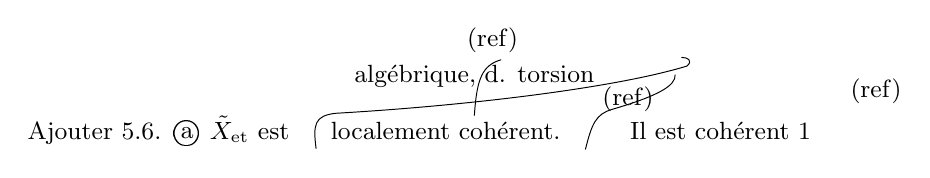
\begin{tikzpicture}[baseline=(a-prefix.base),x=1cm,y=1cm,inner sep=0pt,font=\small]
\node[anchor=base west] (a-prefix) at (0,0) {\uline{Ajouter} 5.6. \textcircled{a} $\tilde{X}_{\mathrm{et}}$ est};
\node[anchor=base west] (a-local) at (3.85,0) {localement cohérent.};
\node[anchor=base west] (a-il) at (7.65,0) {Il est cohérent \deleted{\illegible{1}}};
\node[anchor=base west] (a-add) at (4.15,.72) {\inserted{algébrique, d. torsion}};
\node[anchor=base west] (a-ref-one) at (5.58,1.18) {\inserted{(ref)}};
\node[anchor=base west] (a-ref-two) at (7.30,.43) {\inserted{(ref)}};
\node[anchor=base west] (a-ref-three) at (10.45,.53) {\inserted{(ref)}};
\draw[line width=.35pt] (3.67,-.12) .. controls (3.63,.19) and (3.65,.30) .. (3.92,.33)
  .. controls (5.65,.43) and (7.50,.66) .. (8.38,.93)
  .. controls (8.46,1.00) and (8.39,1.04) .. (8.31,1.04);
\draw[line width=.35pt] (5.68,.30) .. controls (5.71,.77) and (5.78,.94) .. (6.02,1.01);
\draw[line width=.35pt] (7.09,-.13) .. controls (7.17,.19) and (7.22,.32) .. (7.43,.38)
  .. controls (8.01,.55) and (8.24,.68) .. (8.23,.82);
\end{tikzpicture}
(resp. quasi-séparé\inserted{(ref)}) \deleted{\illegible{1}} sss le schéma $X$ est \deleted{\unsure{quasi-cpt|qu.-cpt}} cohérent i.e. qu. cpt qu. \unsure{sép|sep} (resp. quasi-séparé). \deleted{\illegible{1}}}

\handwritten{\textcircled{b} Soit $(X_i)_{i\in I}$ système projectif filtrant à morphismes de transition affines, $X=\varprojlim_i X_i$ (EGA $\overline{\text{\uline{IV}}}$ 8),}

\handwritten{Âlors}
% The corollary is at the right of the conclusion, above En déduire.
\margin{\handwritten{%
\hspace*{-2.2cm}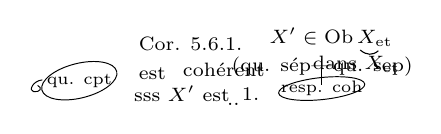
\begin{tikzpicture}[x=.01cm,y=.01cm,baseline=(cor-head.base),inner sep=0pt,font=\fontsize{7}{8}\selectfont]
\node[anchor=base west] (cor-head) at (132,-42) {\uline{Cor.} 5.6.1.};
\node[anchor=base west] (cor-ob) at (298,-34) {$X'\in\mathrm{Ob}\,X_{\mathrm{et}}$};
% Short curved stroke below the et of the first X, with no tilde above X.
\draw[line width=.4pt] (414,-42) .. controls (422,-49) and (430,-49) .. (437,-43);
\node[anchor=base west] at (132,-79) {est};
\node[anchor=base west] at (188,-76) {\deleted{\unsure{cohérent}}};
\node[anchor=base west] at (250,-69) {(\unsure{qu. sép|qu. sep})};
\node[anchor=base west] at (353,-67) {dans $X_{\mathrm{et}}$};
\node[font=\fontsize{6}{7}\selectfont] at (57,-81) {\inserted{qu. cpt}};
\draw[line width=.35pt,rotate around={14:(57,-81)}] (57,-81) ellipse [x radius=49,y radius=22];
\draw[line width=.35pt] (10,-80) .. controls (-2,-81) and (-8,-94) .. (-1,-95)
  .. controls (7,-96) and (11,-90) .. (4,-87);
\node[anchor=base west] at (126,-108) {sss $X'$ est};
\node[anchor=base west] at (244,-112) {..};
\node[anchor=base west] at (263,-106) {\deleted{\illegible{1}}.};
\node[font=\fontsize{6}{7}\selectfont] at (365,-91) {\inserted{resp. coh}};
\draw[line width=.35pt] (365,-54)--(365,-87);
\draw[line width=.35pt,rotate around={6:(365,-91)}] (365,-91) ellipse [x radius=55,y radius=14];
\end{tikzpicture}}}
\[
\handwritten{\tilde{X}_{\mathrm{et}}\simeq\underset{\longleftarrow}{\mathrm{limtop}}\,\tilde{X}_i.}
\]

\handwritten{En \unsure{deduire|déduire} pour 5.7.}

\figure{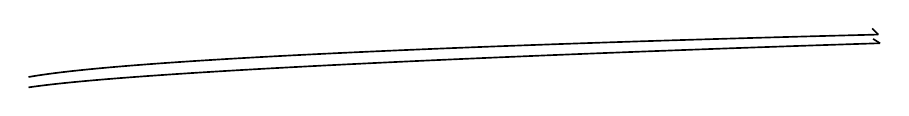
\begin{tikzpicture}[x=.011cm,y=.011cm]
\draw[line width=.6pt] (0,0) .. controls (140,25) and (700,42) .. (981,49);
\draw[line width=.6pt] (974,56)--(981,49);
\draw[line width=.6pt] (0,-12) .. controls (140,9) and (700,30) .. (983,39);
\draw[line width=.6pt] (975,44)--(983,39);
\end{tikzpicture}}

% Isolated faint bent stroke at the left of the pencil reference; function unknown.
\reversemarginpar
\margin{\begin{tikzpicture}[x=1mm,y=1mm]\draw[line width=.3pt] (0,0)--(.1,.7)--(.9,.5);\end{tikzpicture}}
\normalmarginpar
\handwritten{SGA 4 $\overline{\text{\uline{IX}}}$\quad p. 42\qquad note \uline{pour} la p. 8}
\figure{\begin{tikzpicture}[x=.012cm,y=.012cm]
\draw[line width=.4pt] (0,0) .. controls (270,25) and (489,51) .. (697,57)
  .. controls (814,61) and (920,63) .. (1000,67);
\end{tikzpicture}}

\handwritten{$\overline{\text{\uline{VII}}}$\quad 2.1 c)\qquad (p. 9)\quad \uline{corriger}}
% archive sheet number: 23

\scanpage{25}
\figure{\handwritten{%
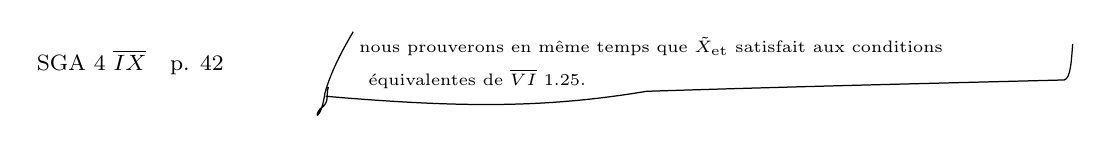
\begin{tikzpicture}[x=.009cm,y=-.009cm,font=\fontsize{8}{9}\selectfont]
\node[anchor=base west] at (160,83) {SGA 4 \(\overline{\text{\uline{IX}}}\)\quad p. 42};
\node[anchor=base west,font=\fontsize{6.5}{8}\selectfont] at (615,57) {nous prouverons en même temps que $\tilde{X}_{\mathrm{et}}$ satisfait aux conditions};
\node[anchor=base west,font=\fontsize{6.5}{8}\selectfont] at (628,104) {équivalentes de \(\overline{\text{\uline{VI}}}\) 1.25.};
\draw[line width=.45pt] (620,28) .. controls (601,60) and (587,89) .. (580,115)
 .. controls (575,151) and (563,151) .. (573,137)
 .. controls (588,128) and (581,117) .. (585,106);
\draw[line width=.45pt] (581,119) .. controls (779,136) and (895,135) .. (1034,112)
 .. controls (1254,105) and (1468,100) .. (1623,96)
 .. controls (1632,94) and (1633,70) .. (1635,45);
\end{tikzpicture}}}

\handwritten{(*) (Note pour la page 8.) Prouvons que la notion de constructibilité 2.3 pour un faisceau d'ensembles $F$ coïncide avec celle de \(\overline{\text{\uline{VI}}}\) 1.9.3. \deleted{Soit} La \deleted{en effet $C$ le \unsure{cas}}\inserted{question étant} locale sur $X$, on peut supposer $X$ affine \inserted{donc ``cohérent'', i.e.} quasi-compact et quasi-séparé. \deleted{Soit $C$ la catégorie \unsure{Soit $C(C')$ le sous-caté|Soit $(C')$ le sous-caté}} \deleted{Je faut alors prouver que $F$ est constructible} Soit $C$ (resp. $C'$) la sous-catégorie \deleted{\unsure{pleine|quasi}}\inserted{strictement} pleine de $\tilde{X}_{\text{ét}}$ formée des $F$ constructibles au sens de 2.3, \deleted{\illegible{1}} \inserted{(resp. au sens de \(\overline{\text{\uline{VI}}}\) 1.9.3), il}}

% The opening conclusion shares the upper-left space of the cancellation graphic.
% The long paths, enclosing edges and nested cross-hatching below are source cancellation marks.

\figure{\handwritten{%
\begin{tikzpicture}[x=.009cm,y=-.009cm,font=\fontsize{6.5}{8}\selectfont]
\node[anchor=base west,rotate=4] at (215,526) {faut prouver};
\node[anchor=base west,rotate=4] at (489,503) {que $C$ s'identifie à la catégorie des objets \uline{cohérents} de};
\node[anchor=base west,rotate=4] at (215,597) {\deleted{$\tilde{X}_{\mathrm{et}}$}};
\node[anchor=base west,rotate=4] at (329,579) {que $C=C'$;};
\draw[line width=.6pt] (490,495)--(1617,425);
\draw[line width=.5pt] (541,497)--(539,576)
 .. controls (521,607) and (526,584) .. (537,578)--(543,518);
\draw[line width=.6pt] (550,496)--(548,601)
 .. controls (533,632) and (537,602) .. (545,594)--(547,552);

\node[anchor=base west,rotate=4] at (574,558) {En vertu de \(\overline{\text{\uline{VII}}}\) 5.6 a),};
\node[anchor=base west,rotate=4] at (1153,515) {\deleted{l'objet final $X$ de} $\tilde{X}_{\mathrm{et}}$};
\node[anchor=base west,rotate=4] at (229,656) {\deleted{est cohérent, donc}};
\node[anchor=base west,rotate=4] at (585,622) {$C'$ est formé des objets \uline{cohérents} \deleted{\(\overline{\text{\uline{VI}}}\)} de $\tilde{X}_{\mathrm{et}}$ (2.5).};
\node[anchor=base west,rotate=4] at (230,708) {En vertu de \(\overline{\text{\uline{VI}}}\) 1.24, \deleted{\unsure{et}} et compte tenu du fait que $C$ est génératrice};
\node[anchor=base west,rotate=4] at (230,784) {dans $\tilde{X}_{\mathrm{et}}$ (2.7.2) et stable par limites inductives finies (2.\unsure{6|8} (i)),};
\node[anchor=base west,rotate=4] at (229,842) {il suffit de prouver que $C\subset C'$,};
\node[anchor=base west,rotate=4] at (941,757) {Mais il résulte de 2.7 que tout};
\node[anchor=base west,rotate=4] at (235,909) {$F\in\mathrm{ob}\,C$ est \uline{quasi-compact}, puisque un};
\node[anchor=base west,rotate=4] at (1065,823) {\deleted{$\unsure{G\in X_{\mathrm{et}}|G\in\mathrm{ob}\,X_{\mathrm{et}}}$ \unsure{représentable par un}}};
\node[anchor=base west,rotate=4] at (1155,784) {\inserted{$\unsure{G|C}\in\unsure{X_{\text{ét}}|X'_{\mathrm{et}}}$}};
\node[anchor=base west,rotate=4] at (231,983) {\deleted{schéma $X'\unsure{\in|C}$} qui est quasi-compact et quasi-séparé est quasi-compact};
\node[anchor=base west,rotate=4] at (229,1046) {comme objet de $\tilde{X}_{\mathrm{et}}$ \deleted{(5.6.1)} (\(\overline{\text{\uline{VII}}}\) 5.6.1).};

\node[anchor=base west,rotate=4] at (1151,952) {D'autre part pour};
\node[anchor=base west,rotate=4] at (233,1099) {\unsure{voir que} $\unsure{F|F'}\unsure{\in|\to}\unsure{\mathrm{ob}\,X'|X'}$ la diagonale};
\node[anchor=base west,rotate=4] at (1069,1020) {$\unsure{F\longrightarrow F\mathbin{\times}_{X}F|F\longrightarrow F\mathbin{\times}F}$ est quasi-compacte,};
\node[anchor=base west,rotate=4] at (231,1172) {il suffit de voir que \unsure{pour tout} \illegible{2}};
\node[anchor=base west,rotate=4] at (232,1238) {\unsure{et que}\illegible{2} \unsure{ce fait que $C$ est stable par produits}};
\node[anchor=base west,rotate=4] at (744,1156) {Comme $C$ est stable par};
\node[anchor=base west,rotate=4] at (1321,1097) {\deleted{limites projectives}};
\node[anchor=base west,rotate=4] at (1393,1062) {\inserted{produits}};
\node[anchor=base west,rotate=4] at (340,1248) {\inserted{(2.6 (ii))}};
\node[anchor=base west,rotate=4] at (243,1297) {finis, l'inclusion $C\subset C'$ est donc un cas particulier de 2.1.};

% Left oval aligned with its source position inside the cancelled proof.
\begin{scope}[shift={(29,924)}]
\node[font=\tiny,anchor=center,align=center,rotate=28] at (98,85) {\unsure{pourquoi|pourq.|pour}\\par exemple};
\draw[line width=.4pt] (20,68) .. controls (56,18) and (108,3) .. (148,23)
 .. controls (189,42) and (177,90) .. (152,113)
 .. controls (105,153) and (47,176) .. (12,153)
 .. controls (0,136) and (4,96) .. (20,68);
\draw[line width=.5pt] (15,72)--(121,161);
\draw[line width=.5pt] (47,42)--(154,132);
\draw[line width=.5pt] (113,16) .. controls (127,60) and (147,92) .. (162,110);
\draw[line width=.5pt] (145,23)--(184,48);
\end{scope}

% Irregular enclosing edges and long oblique cancellation strokes.
\draw[line width=.6pt] (235,649)--(545,616);
\draw[line width=.5pt] (238,650)--(239,1219)--(252,1294)--(1598,1158)
 .. controls (1625,1157) and (1645,1112) .. (1650,1092);
\draw[line width=.5pt] (235,884)--(979,798)--(941,801)--(942,745)--(1591,697);
\draw[line width=.55pt] (239,646)--(586,1217);
\draw[line width=.55pt] (512,623)--(885,1222);
\draw[line width=.55pt] (624,480)--(1151,1198);
\draw[line width=.55pt] (917,472)--(1365,1170);
\draw[line width=.55pt] (1148,452)--(1602,1100);
\draw[line width=.55pt] (1418,452)--(1645,797);
\draw[line width=.45pt] (1556,429)--(1643,535);

% Nested cancelled attempt: right-hand band, lower-left band, and its tail.
\draw[line width=.6pt] (1156,929)--(1599,886)
 .. controls (1610,887) and (1610,922) .. (1618,943);
\draw[line width=.6pt] (1611,947)--(1610,1007)
 .. controls (1590,1029) and (1590,1006) .. (1608,1003);
\draw[line width=.55pt] (1610,1014)--(951,1086)--(952,1024)--(230,1075)--(222,1164)--(705,1110)--(704,1189)--(236,1233);
\draw[line width=.5pt] (228,1077)--(313,1147);
\draw[line width=.5pt] (244,1156)--(301,1069);
\draw[line width=.5pt] (289,1073)--(373,1140);
\draw[line width=.5pt] (316,1148)--(365,1060);
\draw[line width=.5pt] (359,1065)--(442,1130);
\draw[line width=.5pt] (386,1137)--(435,1053);
\draw[line width=.5pt] (430,1057)--(514,1122);
\draw[line width=.5pt] (459,1130)--(507,1047);
\draw[line width=.5pt] (501,1048)--(586,1113);
\draw[line width=.5pt] (532,1123)--(579,1039);
\draw[line width=.5pt] (572,1040)--(659,1105);
\draw[line width=.5pt] (605,1116)--(652,1032);
\draw[line width=.5pt] (645,1033)--(731,1097);
\draw[line width=.5pt] (678,1107)--(725,1023);
\draw[line width=.5pt] (718,1025)--(806,1089);
\draw[line width=.5pt] (751,1100)--(800,1016);
\draw[line width=.5pt] (793,1017)--(880,1081);
\draw[line width=.5pt] (824,1091)--(875,1009);
\draw[line width=.5pt] (868,1009)--(951,1073);
\draw[line width=.5pt] (897,1084)--(947,1001);
\draw[line width=.5pt] (1158,933)--(1251,989);
\draw[line width=.5pt] (1179,995)--(1241,924);
\draw[line width=.5pt] (1231,925)--(1336,977);
\draw[line width=.5pt] (1283,986)--(1330,914);
\draw[line width=.5pt] (1318,918)--(1420,969);
\draw[line width=.5pt] (1366,977)--(1418,906);
\draw[line width=.5pt] (1409,908)--(1506,958);
\draw[line width=.5pt] (1454,970)--(1499,899);
\draw[line width=.5pt] (1498,899)--(1599,946);
\draw[line width=.5pt] (1538,962)--(1584,903);
\draw[line width=.45pt] (258,1224)--(464,1139);
\draw[line width=.45pt] (402,1209)--(665,1119);
\end{tikzpicture}}}

\handwritten{En vertu de \(\overline{\text{\uline{VI}}}\) 2.9, b), il suffit de voir que $C$ est stable pour limites inductives finies et limites projectives finies, qu'elle est génératrice, et formée d'objets quasi-compacts. \deleted{\unsure{Et|et}} Compte tenu de 2.6 (i) et (2.7.2), il reste à prouver que tout $F\in\mathrm{ob}\,C$ est quasi-compact. Or 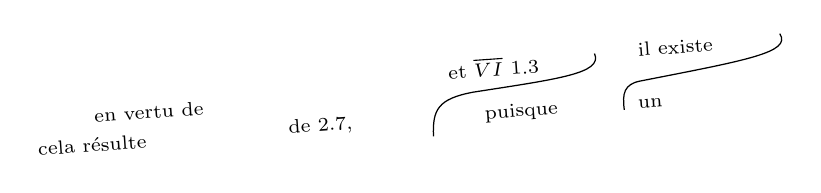
\begin{tikzpicture}[baseline=(correctionbase.base),x=.014cm,y=-.014cm,font=\scriptsize]
\node[anchor=base west,rotate=4] at (270,1578) {\deleted{cela résulte}};
\node[anchor=base west,rotate=4] at (321,1548) {\inserted{en vertu de}};
\node[anchor=base west,rotate=4] at (497,1558) {de 2.7,};
\node[anchor=base west,rotate=4] at (642,1509) {\deleted{et \(\overline{\text{\uline{VI}}}\) 1.3}};
\node[anchor=base west,rotate=4] at (675,1545) {\deleted{puisque}};
\node[anchor=base west,rotate=4] at (814,1488) {\inserted{il existe}};
\node[anchor=base west,rotate=4] (correctionbase) at (814,1535) {un};
\draw[line width=.45pt] (783,1485) .. controls (791,1503) and (750,1508) .. (673,1520)
 .. controls (641,1526) and (636,1536) .. (637,1560);
\draw[line width=.45pt] (951,1467) .. controls (962,1484) and (921,1491) .. (824,1510)
 .. controls (810,1513) and (808,1521) .. (810,1536);
\end{tikzpicture} $G\in\mathrm{ob}\,X_{\mathrm{et}}$ \deleted{et} qui est \inserted{un schéma} quasi-compact et quasi-séparé \deleted{\unsure{et} est} et un épimorphisme $G\longrightarrow F$. Or $G$ \deleted{\unsure{comme on}} est un objet quasi-compact de $\tilde{X}_{\text{ét}}$ (\(\overline{\text{\uline{VII}}}\) 5.6.1), donc $F$ est quasi-compact (\(\overline{\text{\uline{VI}}}\) 1.3), qfd.}

\handwritten{Bien entendu, il y aurait \inserted{eu} lieu de refondre les §§ 1,2 du présent exposé, \inserted{notamment} en les rattachant \inserted{\deleted{\unsure{explicitement}}} aux notions générales de \deleted{l'exposé} finitude de \(\overline{\text{\uline{VI}}}\). Nous laissons ce soin \deleted{\unsure{complémentaire}} de rédaction aux générations futures.}
% archive sheet number: 24

\scanpage{27}
\mspage{\handwritten{19}}
% Source viewed upright after a 180-degree rotation.
% The enclosing TikZ reconstruction carries the page-wide cancellation strokes.
% Ordinary local cancellations remain \deleted; the whole draft is cancelled
% by the drawn oblique strokes, rather than by an invented horizontal strike.
% The left marginal oval is placed in the same coordinate system as its line.
\reversemarginpar
\figure{%
\begingroup
\csname tagsleft@true\endcsname
\begin{tikzpicture}[x=.01cm,y=-.01cm,scale=.74,transform shape,
  every node/.style={anchor=north west,inner sep=0pt,align=left,
    font=\fontsize{10}{20}\selectfont\ttfamily}]
\path[use as bounding box] (55,180) rectangle (1650,2145);

\node at (230,202) {\begin{minipage}{14.1cm}
2.1.1.\quad On peut dire encore qu'une structure de biextension sur le $G_{P\times Q}$-torseur $E$ est définie par deux lois de composition non partout définies $\handwritten{\phi}(x,y)$ et $\handwritten{\psi}(x,y)$ sur $E$, la première étant définie lorsque \deleted{$j($} $\mathrm{pr}_2j(x)=\mathrm{pr}_2j(y)$, la deuxième lorsque $\mathrm{pr}_1j(x)=\mathrm{pr}_1j(y)$ \deleted{(où} (où $j:E\handwritten{\longrightarrow}P\times Q$ est le morphisme structural du torseur). Les axiomes, en plus des associativités du type
\end{minipage}};

\node[anchor=center] at (107,374) {$\handwritten{\unsure{\psi|\Psi}}$};
\draw[line width=.45pt] (116,324) .. controls (87,324) and (58,389) .. (74,424)
  .. controls (91,454) and (145,391) .. (139,351)
  .. controls (138,339) and (128,329) .. (116,324);

% Two small isolated ink dots at the left of the abandoned formula.
\fill (237,633) circle[radius=.014cm];
\fill (233,640) circle[radius=.014cm];

\node at (465,616) {\begin{minipage}{8.35cm}
\[
\deleted{\handwritten{\phi}(gx,y)\unsure{=}g\handwritten{\phi}(x,y),\quad\handwritten{\phi}(x,gy)\unsure{=}g\handwritten{\phi}(x,y),\quad\handwritten{\phi}(}
\]
\end{minipage}};

\node at (230,666) {\begin{minipage}{14.1cm}
\[
\handwritten{\phi}(gx,y)=\handwritten{\phi}(x,gy)=g\handwritten{\phi}(x,y)\qquad(x,y\handwritten{\in}E(S),\ g\handwritten{\in}G(S))
\tag*{(2.1.1.1)}
\]
\end{minipage}};

\node at (230,751) {\begin{minipage}{14.1cm}
et des relations analogues en $\handwritten{\psi}$, s'expriment alors par l\deleted{a}'associativité et la commutativité de \unsure{\deleted{s}c|\deleted{c}s}es lois de composition partielles, et par la relation
\end{minipage}};

\node at (230,946) {\begin{minipage}{14.1cm}
\[
\handwritten{\phi}(\handwritten{\psi}(x,y),\handwritten{\psi}(z,t))=\handwritten{\psi}(\handwritten{\phi}(x,z),\handwritten{\phi}(y,t))
\tag*{\raisebox{10pt}{(2.1.1.2)}}
\]
\end{minipage}};
% The two local hooked strokes are distinct from the page-wide cancellation.
\draw[line width=.45pt] (301,1005) .. controls (281,982) and (436,953) .. (562,941) -- (565,928);
\draw[line width=.6pt] (441,934) .. controls (465,950) and (421,966) .. (399,982)
  .. controls (382,994) and (399,1010) .. (424,1018)
  .. controls (472,1022) and (522,1018) .. (571,1021) -- (574,1034);

\node at (230,1039) {\begin{minipage}{14.1cm}
pour $x,y,z,t$ respectivement dans $E_{p,q}(S),E_{p,q'}(S),E_{p',q}(S),E_{p',q'}(S)$.
\end{minipage}};

\node at (350,1088) {\inserted{\handwritten{\uline{Sections unité}.}}};
\draw[line width=.45pt] (652,1107) .. controls (659,1134) and (601,1135) .. (444,1136)
  .. controls (423,1134) and (412,1151) .. (418,1167);

\node at (230,1126) {\begin{minipage}{14.1cm}
2.2.\quad Il y a lieu de considérer la section unité de $\mathbb{E}\deleted{t}$ considéré comme extension de $Q_P$ par $G_P$,
\end{minipage}};

\node at (230,1252) {\begin{minipage}{14.1cm}
\[
e_{E/P}\handwritten{\in\Gamma}(E/P)=\mathrm{Hom}_P(P,E)\ ,
\tag*{(2.2.1)}
\]
\end{minipage}};

\node at (230,1334) {\begin{minipage}{14.1cm}
et de façon symétrique la section unité de $E$\handwritten{,} considéré comme extension de $P_Q$ par $G_Q$,
\end{minipage}};

\node at (230,1462) {\begin{minipage}{14.1cm}
\[
e_{E/Q}\handwritten{\in\Gamma}(E/Q)=\mathrm{Hom}_Q(Q,E)\ .
\tag*{(2.2.2)}
\]
\end{minipage}};

% This is one paragraph. Its two interlinear additions are placed separately
% at their source positions so that their relation to the cancellation is kept.
\node at (230,1547) {\begin{minipage}{14.1cm}
En particulier, \uline{le torseur} $E$ \uline{au dessus de} $P\times Q$ (de \unsure{\deleted{g}G|\deleted{G}g}roupe $G_{P\times Q}$) \uline{est canoniquement trivialisé au dessus de} $1_P\times Q$ \uline{par} $e_{E/P}$, \uline{et au dessus de} $P\times1_Q$ \uline{par} $e_{E/Q}$. \uline{\unsure{\deleted{C}c|\deleted{c}C}es deux trivialisations coïncident au dessus de la section unité} $1_P\times1_Q$ \uline{de} $P\times Q$, et définissent une même section
\end{minipage}};
\node at (590,1654) {\inserted{De plus,}};
\node at (591,1676) {\deleted{\handwritten{\illegible{1}}}};
\draw[line width=.6pt] (767,1668) .. controls (780,1699) and (645,1682) .. (600,1687)
  .. controls (569,1690) and (571,1715) .. (578,1734);
\node at (1071,1728) {\inserted{\handwritten{donc}}};
\draw[line width=.45pt] (1153,1738) .. controls (1169,1756) and (1082,1752) .. (1085,1781);

\node at (230,1819) {\begin{minipage}{14.1cm}
\[
e_{E\deleted{/S}}\handwritten{\in\Gamma}(E\handwritten{)}\deleted{\unsure{/S)|/P)|/Q)}}\ ,
\tag*{(2.2.3)}
\]
\end{minipage}};

\node at (230,1898) {\begin{minipage}{14.1cm}
qu'on appellera par abus de langage la \uline{section unité} (ou \uline{section neutre}) de $E$. Pour prouver l'égalité annoncée\deleted{, et une conséquence} des deux sections $e,e'$ de $E$ déduites respectivement de $e_{E/P}$ et $e_{E/Q}$, on note
\end{minipage}};

% Page-wide source strokes; upright coordinates in the original 1685 x 2159 scan.
\draw[line width=.65pt] (1495,351) .. controls (1230,570) and (455,1360) .. (132,1740);
\draw[line width=.55pt] (1555,998) .. controls (1270,1275) and (765,1828) .. (522,2120);
\draw[line width=.5pt] (1558,1427) .. controls (1613,1510) and (1290,1933) .. (1118,2110);
\draw[line width=.45pt] (495,188) .. controls (585,317) and (1005,1260) .. (1235,1892);
\draw[line width=.4pt] (938,238) .. controls (1056,501) and (1400,1065) .. (1485,1420);
\draw[line width=.4pt] (220,623) .. controls (218,864) and (445,1770) .. (435,2140);
\end{tikzpicture}
\endgroup
}
\normalmarginpar
% archive sheet number: 26 (oppositely oriented to the typescript)

\scanpage{30}
\reversemarginpar
\margin{\handwritten{SGA 4 $\overline{\text{\uline{XVI}}}$}}
\normalmarginpar
\mspage{VII 2}

Du point de vue substance, 2.1.1 se ramène trivialement au cas où dans $X\handwritten{\longrightarrow}S$, $X$ est affine, donc quasi-compact quasi-séparé (on dit maintenant ``cohérent''), et alors c'est une conséquence du th. de changement de base par $f$, qui est donné dans SGA \unsure{\deleted{V}4|\deleted{4}V} XVI 1.1\inserted{et qui est essentiellement}. Mais dans loc. cit. on utilise toute la force du théorème de changement de base propre, ce qui est en effet abusif, car en interprétant comme un énoncé d'acyclicité globale 2.1.1, on est ramené comme tu l'observes \deleted{à 2.1.5} au cas particulier 2.1.5, qui se ramène trivialement à son tour au cas du degré de transcendance 1, et par là au th.\unsure{\handwritten{,}} de changement de\inserted{corps de} base pour le $H^1$ premier à $p$ pour une courbe propre et lisse. Je pense présenter les choses ainsi en réédition de SGA 4, de sorte que ton 2.1.1 y sera énoncé en toutes lettres, s'il ne l'est déjà (je n'ai pas les textes en main).
\reversemarginpar
\margin{\figure{\handwritten{\begin{tikzpicture}[x=.012cm,y=.012cm]
\draw[line width=.25pt] (0,0) .. controls (30,-8) and (43,-7) .. (63,12) .. controls (77,27) and (89,43) .. (97,54);
\end{tikzpicture}}}}
\normalmarginpar
Cela te dispensera donc de le prouver, ta seule tâche consistant à interpréter en termes de champs cet énoncé \deleted{(que tu pourrais donner sous forme de rappels)}.

Du point de vue rédaction, on a l'impression que tu t'es ingénié à tout présenter à l'\unsure{\(\mathbb{e}\)|\deleted{E}e|\deleted{e}E}nvers. Il faut en tous cas bloquer ensemble 2.1.1 et 2.1.7 (pratiquement identiques) et 2.1.5 (celui-ci en corollaire, peut-être)
% The following connected cancellation is drawn in its observed geometry.
% Its source origin is approximately (225,1507). The semantic state macros
% retain the cancelled/underlined text; their automatic lines are suppressed
% locally because the actual border, obliques and underlines are drawn below.
% BEGIN cancellation graphic
\begingroup
\renewcommand{\ULthickness}{0pt}
\figure{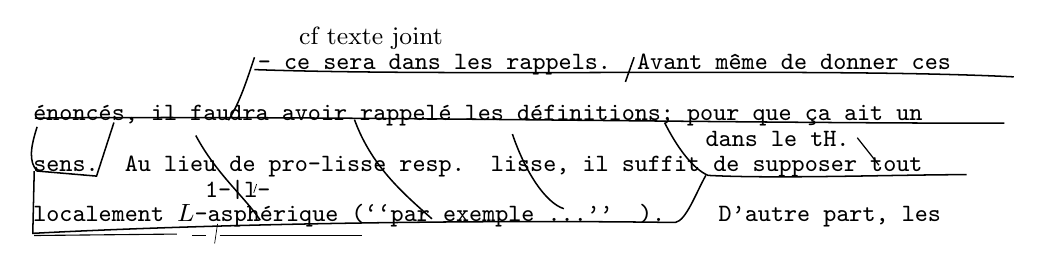
\begin{tikzpicture}[x=.0092cm,y=-.0092cm,every node/.style={inner sep=0pt,anchor=base west,font=\small\ttfamily}]
\node at (310,0) {\deleted{- ce sera dans les rappels\unsure{.} Avant même de donner ces}};
\node[font=\small] at (367,-34) {\inserted{\handwritten{cf texte joint}}};
\node at (0,70) {\deleted{énoncés, il faudra avoir rappelé les définitions; pour que ça ait un}};
\node at (0,140) {\deleted{sens. Au lieu de pro-lisse resp. lisse, il suffit de supposer tout}};
\node at (928,106) {\deleted{\inserted{dans le tH.}}};
\node at (237,177) {\deleted{\inserted{\unsure{1-|l-}}}};
\node at (0,210) {\deleted{\uline{localement} \uline{$L$}-\uline{asphérique} (``par exemple ...'' )}.};
\node at (946,210) {D'autre part, {\renewcommand{\ULthickness}{.4pt}\deleted{les}}};
\draw[line width=.55pt] (306,-17) .. controls (296,13) and (286,45) .. (270,70);
\draw[line width=.55pt] (306,0) .. controls (590,10) and (1090,-3) .. (1354,10);
\draw[line width=.55pt] (830,-17)--(818,17);
\draw[line width=.55pt] (3,67) .. controls (368,63) and (941,74) .. (1341,74);
\draw[line width=.55pt] (6,79) .. controls (-3,107) and (-6,127) .. (6,140)--(88,147)--(112,73);
\draw[line width=.55pt] (2,140)--(0,226) .. controls (247,213) and (600,207) .. (887,211) .. controls (902,208) and (915,171) .. (929,146);
\draw[line width=.55pt] (225,91) .. controls (254,145) and (293,176) .. (314,208);
\draw[line width=.55pt] (444,69) .. controls (467,132) and (509,169) .. (551,206);
\draw[line width=.55pt] (662,89) .. controls (680,142) and (708,184) .. (733,192);
\draw[line width=.55pt] (872,73) .. controls (889,107) and (911,137) .. (932,146) .. controls (1027,151) and (1191,145) .. (1289,145);
\draw[line width=.45pt] (1138,94)--(1168,132);
\draw[line width=.4pt] (2,229)--(199,227);
\draw[line width=.4pt] (220,229)--(239,229);
\draw[line width=.4pt] (258,229)--(454,229);
\draw[line width=.25pt] (309,158)--(305,170);
\draw[line width=.25pt] (255,213)--(251,240);
\end{tikzpicture}}
\endgroup
% END cancellation graphic
\reversemarginpar
\margin{\handwritten{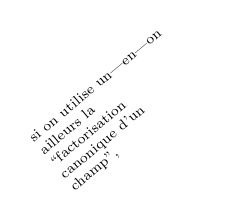
\begin{tikzpicture}[scale=.72,transform shape]
\node[rotate=40,anchor=south west,align=left,inner sep=0pt,font=\scriptsize] at (0,0) {\unsure{si on utilise} \unsure{un|en|on}\\ailleurs la\\``factorisation\\\unsure{c}anonique d'un\\champ'',};
\end{tikzpicture}}}
\normalmarginpar
\deleted{énoncés} 2.12, 2.1.3, 2.1.4, 2.1.7.1 n'ont rien à voir avec les schémas, il sont manifestement importants en eux-mêmes et devraient passer dans un numéro à part dans
% BEGIN reference correction
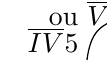
\begin{tikzpicture}[baseline=(iv.base),x=.01cm,y=.01cm]
\node[inner sep=0pt,anchor=base west] (iv) at (0,0) {\handwritten{$\overline{\text{\uline{IV}}}$}};
\node[inner sep=0pt,anchor=base west] at (47,0) {\deleted{5}};
\node[overlay,inner sep=0pt,anchor=base west] at (27,34) {\inserted{\handwritten{ou $\overline{\text{\uline{V}}}$}}};
\draw[overlay,line width=.45pt] (76,-10) .. controls (81,26) and (92,36) .. (126,45) .. controls (143,51) and (150,57) .. (152,65);
\end{tikzpicture}
% END reference correction
(avec un peu d'ordre dans la suite des énoncés)

% BEGIN final cancelled line
\figure{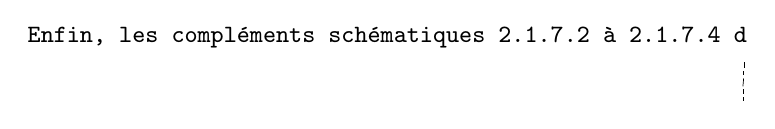
\begin{tikzpicture}[x=.0092cm,y=-.0092cm]
\node[inner sep=0pt,anchor=base west,font=\small\ttfamily] at (0,0) {\deleted{Enfin, les compléments schématiques 2.1.7.2 à 2.1.7.4 d}};
\draw[line width=.25pt] (990,27)--(990,34);
\draw[line width=.25pt] (989,39)--(989,45);
\draw[line width=.25pt] (989,49)--(988,60);
\draw[line width=.25pt] (988,64)--(988,70);
\draw[line width=.25pt] (988,75)--(988,80);
\end{tikzpicture}}
% END final cancelled line
% archive sheet number: 29
